%!TEX root = flock-comment-main.tex

\section*{Introduction}
Methods for the unsupervised clustering of genotypes have received 
considerable attention in the molecular ecology literature.  
The best known example of this class of methods is {\sc structure} 
\citep{Pritchardetal2000}, with over 12,000 citations identified on 
Google Scholar.  A variety of other 
clustering methods have been developed that are all closely related to 
{\sc structure}, for example {\sc NewHybrids} \citep{And&Tho2002}, {\sc 
BayesAss+} \citep{Wil&Ran2003}, and {\sc baps} 
\citep{Coranderetal2004}. An overview of the similarities between these methods can be 
found in \citet{Anderson2009PGAC}.

Recently, several colleagues suggested we try using the software {\sc flock} \citep{Duc&Tur2009},
for analyzing a number of the data sets from our laboratories.
{\sc flock} is billed as a ``non-Bayesian method [that] 
differs substantially from previous 
clustering algorithms'' \citep[][p.~1333]{Duc&Tur2009}. As described
in a later paper, {\sc flock} ``does not sample the space of partitions through small 
random step walks as in MCMC, and it does not try to optimize some 
target function, such as HWLE\@. Briefly stated, it is not based on a 
probabilistic search algorithm. On the contrary, {\sc flock} is 
entirely deterministic'' \citep[][p.~736]{Duc&Tur2012}.

In trying to understand the behavior of {\sc flock} we identified 
a close relationship between {\sc flock}'s algorithm and the program
{\sc structure}.  In other words, although the algorithm in {\sc flock}
is, as the authors point out, entirely deterministic, it can be interpreted as a 
limiting case of a probabilistic search algorithm applied to one of {\sc structure}'s
models.  More specifically, the {\sc flock} 
algorithm is a special case of the simulated annealing
algorithm for finding the Bayesian maximum-{\em a-posteriori}
estimate from a marginalized form of the {\sc structure} model with no
admixture and non-correlated allele frequencies.  

Being able to interpret {\sc flock} in this fashion should help users
interpret output from {\sc flock} and predict when it might and might not
give substantially different results than {\sc structure}. Below we describe
the correspondence between the programs in more detail, and then, for illustration, compare
the results obtained from {\sc flock} and {\sc structure} on a large, real data
set.

\section*{Comparison of methods}
We start with a succinct mathematical description of the {\sc structure}
model, then describe the {\sc flock} algorithm, and finally explain
the close relationship between the two.


\subsection*{{\sc structure}}
In the {\sc structure} model with no admixture (which, it should be pointed out, 
is not the default model in {\sc structure}), the unknown ``subpopulation'' that the 
$i\thh$ individual ($i=1,\ldots,N)$ belongs to is denoted by $Z_i \in \{1,\ldots,K\}$, 
where $K$ is the 
number of subpopulations (or clusters, as they are often referred to).  
In a diploid individual from cluster $k$, the 
allelic types of the two gene copies at the $\ell\thh$ locus are assumed
to be drawn independently from the vector of allele frequencies at
locus $\ell$ in subpopulation $k$,  $\theta_{k\ell}=(\theta_{k\ell 1},\ldots,\theta_{k\ell A_\ell})$, where 
$A_\ell$ 
denotes the number of alleles observed in the data set at locus $\ell$.
Hence, if $Y_{i\ell}$ denotes a vector of length $A_\ell$ whose components denote the 
number
of copies of each of the $A_\ell$ alleles at locus $\ell$ in a diploid individual $i$, and 
$Z_i=k$, then $Y_{i\ell}$ follows the multinomial distribution of two trials with
$A_\ell$  components and cell probabilities given by the allele frequencies: 
\begin{equation}
(Y_{i\ell}~|~Z_i=k) \sim \mathrm{Mult}_{A_\ell}(2, \theta_{k\ell}).
\end{equation}
In the {\sc structure} model without physical linkage, the genotypes at the loci are assumed to
be independent of one another, so the probability of the genotype data at
all $L$ loci---$Y_i=(Y_{i1},\ldots,Y_{iL})$---is simply a product of multinomial 
probabilities.
In the uncorrelated allele frequencies model, the prior on each $\theta_{k\ell}$ is a
Dirichlet distribution with parameters $(\lambda_{k\ell1},\ldots,\lambda_{k\ell A_
\ell})$,
which are usually all set to a value such as 1 or $1/A_\ell$.  

After initializing the unknown allele frequencies, $\theta = (\theta_1,\ldots,\theta_K)$, to randomly drawn values,
$\theta^{(0)}$, inference in the model proceeds by sampling from the joint posterior of the 
$Z_i$'s and $\theta$ using Gibbs sampling.  That is,
at iteration $t = 0, 1, 2, \ldots$:
\begin{enumerate}
\item each $Z^{(t)}_i$ is updated to $Z^{(t+1)}_i$ by sampling a value from 
the full conditional distribution of $Z_i$ given
$Y_i$ and $\theta^{(t)}$ (the current estimate of the allele frequencies).  This
distribution is found using Bayes' theorem. In {\sc structure}'s formulation, the 
prior probability that $Z_i=k$ is $1/K$ for all $k=1,\ldots, K$.     
\item $\theta^{(t)}$ is updated to $\theta^{(t+1)}$ from its full conditional distribution.  For each 
cluster
$k$ and locus $\ell$, the full conditional for $\theta_{k\ell}$ is independently a 
Dirichlet distribution with parameters $\lambda_{k\ell j} + \#(k,\ell,j)$, for 
$j=1,\ldots, A_\ell$,
where $\#(k,\ell,j)$ is the number of alleles of type $j$ at locus $\ell$ observed in 
individuals with $Z^{(t+1)}_i = k$.   
\end{enumerate}

It will be useful for our comparison with {\sc flock} to point out that another way 
of pursuing inference in this model would be to first integrate out the 
Dirichlet priors on the allele frequencies and then sample from the posterior
for the $Z_i$'s by Gibbs sampling.  When $\theta$ is integrated out, the genotypes 
of the individuals are no longer conditionally independent (they were originally
independent {\em conditional} on $\theta$ and the $Z_i$'s), so the calculation of 
the full conditional distribution of $Z_i$ becomes somewhat more involved,
but can be computed by the following reasoning. First, the 
conditional distribution of $Y_{i\ell}$, given that individual $i$ is from subpopulation $k$
(\ie $Z_i=k$), depends on the 
cluster memberships and genotypes  of all the remaining individuals,
which we denote by  $Z_{(-i)}$ and $Y_{(-i)\ell}$, respectively.
This full conditional for $Y_{i\ell}$ follows 
a Compound Dirichlet Multinomial distribution (CDM):
\begin{eqnarray}
\lefteqn{(Y_{i\ell}~|~Z_i=k,~Z_{(-i)},~Y_{(-i)\ell}) \sim} \label{eq:cdm}\\
& & \mathrm{CDM}(\lambda_{k\ell 1} + \#_{(-i)}(k,\ell,1), \ldots,
\lambda_{k\ell A_\ell} + \#_{(-i)}(k,\ell,A_\ell)), \nonumber
\end{eqnarray}
where $\#_{(-i)}(k,\ell,j)$ is the number of alleles of type $j$ at locus $\ell$
found in individuals {\em other than individual $i$} that currently
belong to cluster $k$. Thus, calculating (\ref{eq:cdm}) for each value of $Z_i=k \in 
\{1,\ldots,K\}$ 
and normalizing to sum to one gives the full conditional distribution for 
$Z_i$:
\begin{equation}
P(Z_i=k~|~Y_i, ~Z_{(-i)},~Y_{(-i)\ell})~~,~~k=1,\ldots,K.
\label{eq:fc}
\end{equation}
A new value of $Z_i$ would be drawn from (\ref{eq:fc}) if doing Gibbs sampling in this
version of the {\sc structure} model in which $\theta$ has been integrated out.  In 
fact,
this is the approach (with a slightly different prior weight on the $Z_i$'s) taken to 
update 
$Z_i$ in both {\sc hwler} \citep{Pel&Mas2006} and {\sc structurama} \citep{Hue&And2007} 
when not
proposing changes to the number of clusters.



\subsection*{{\sc flock}}
Here we translate the recipe given by \citeauthor{Duc&Tur2009} for the 
{\sc flock} algorithm into a specification in terms of the variables
defined in the previous section.  We provide the description for a case in which
it is assumed there are $K$ clusters.

The first step of the flock algorithm is initialization, during which 
the program randomly allocates each of the $N$ individuals to one of 
$K$ clusters.  Then a number of reallocation steps are performed.  During every one of 
these steps, each individual is given the chance to be reallocated 
(\ie moved to a different cluster).  This is done on the basis of 
maximum likelihood: as \citeauthor{Duc&Tur2009} say (2009, p.~1335), ``Re-allocations are 
performed following multilocus maximum likelihood (Paetkau et al. 1995).''

From that description, it is not clear how \citeauthor{Duc&Tur2009} treat 
alleles that appear in the focal
individual but do not appear within any other individuals within a cluster.
The original approach of \citet{Paetkauetal1995} merely added 0.01 or some other
small value to each allele frequency that was 0, and then renormalized 
the allele frequencies to sum to 1.  In later works, Paetkau and colleagues
also employed the ``Bayesian'' approach of \citet{Ran&Mou1997} in their 
software {\sc geneclass2}  \citep{Piryetal2004}.  If \citeauthor{Duc&Tur2009}
use the approach of \citet{Ran&Mou1997}, then the $i\thh$ individual will
be reallocated to whichever cluster gives the highest value to 
$P(Y_{i\ell}~|~Z_i=k,~Z_{(-i)},~Y_{(-i)\ell})$, which is exactly the probability
defined in (\ref{eq:cdm}).  
If \citeauthor{Duc&Tur2009} use the simpler ``add 0.01 and renormalize''
formulation of \citet{Paetkauetal1995}, then their reallocations are based
on maximizing a likelihood that, although it may not be formally identical to
that in (\ref{eq:cdm}), is nearly identical to it.   

It is worth pointing out that, since the
{\sc structure} model without admixture assumes a uniform prior over 
the $K$ different clusters, $P(Y_{i\ell}~|~Z_i=k,~Z_{(-i)},~Y_{(-i)\ell})$
is exactly proportional to $P(Z_i=k~|~Y_i, ~Z_{(-i)},~Y_{(-i)\ell})$, which 
we have shown is the
full conditional distribution for $Z_i$ in the {\sc structure} model after
integrating out $\theta$.  Thus, we have shown that, doing Gibbs
sampling for $Z_i$ in  the {\sc structure} model in which $\theta$ has been
integrated out would involve sampling a new value of $Z_i$ from the 
probability distribution,
\[
P(Z_i=k~|~Y_i, ~Z_{(-i)},~Y_{(-i)\ell})
\]
and that the updates that
{\sc flock} makes to each $Z_i$ involve assigning to $Z_i$
\begin{equation}
\arg\max_k P(Z_i=k~|~Y_i, ~Z_{(-i)},~Y_{(-i)\ell}),
\end{equation}
\ie the value of $k$ that maximizes $P(Z_i=k~|~Y_i, ~Z_{(-i)},~Y_{(-i)\ell})$
(or, as stated above, a nearly identical function of $k$, depending on how
the program {\sc flock} treats alleles that are not observed in certain clusters).






\subsection*{The {\sc flock} algorithm and {\sc structure}}
The goal of {\sc structure}'s MCMC algorithm is to sample from the space of 
$Z$'s in proportion to their posterior probability.  If, all that was desired
was a point estimate of the $Z_i$'s that maximized the posterior probability,
then one standard approach to finding that maximum-{\em a-posteriori}, or MAP, 
estimate, would be to use simulated annealing \citep{Kirkpatricketal1983}.
To do simulated annealing in the {\sc structure} model with no admixture and
no correlated allele frequency prior, after integrating out the unknown
allele frequencies, the updates for each $Z_i$ would be made from the 
distribution
\[
\biggl[P(Z_i=k~|~Y_i, ~Z_{(-i)},~Y_{(-i)\ell})\biggr]^\beta
\]
which is the same full conditional distribution as the marginalized {\sc structure}
model (equation~\ref{eq:fc}), raised
to the power $\beta$.  In typical applications of simulated annealing,
$\beta$ is set to a starting value less than 1, and, as the algorithm proceeds,
$\beta$ is increased according to a ``cooling schedule''\citep{Hajek1988}, until
the algorithm finds a local maximum in the posterior probability surface.  
When $\beta$ is small, the process can easily traverse ``valleys''
in the posterior probability surface and has a better chance of searching
more of the space for the maximum value.  As $\beta$ gets larger, it becomes
more probable that the process will
move uphill on the probability surface, tending toward the local
maximum near where it currently is.    

It should now be clear that the algorithm in {\sc flock} is a simulated annealing 
algorithm for the {\sc structure} model in which the cooling schedule is
``start with $\beta\rightarrow\infty$ and leave it there for the duration of 
the algorithm.''  As such, we can expect that it may be more susceptible 
to becoming trapped in local modes of the posterior probability. 
In the following section we show that {\sc structure} and {\sc flock} find similar
solutions in the analysis of a large microsatellite data set, though, as expected,
{\sc flock} seems to find the same solution less consistently than does {\sc structure}.





\section*{Comparison of {\sc structure} and {\sc flock} results}

We used a published dataset of 2596 steelhead, \textit{Oncorhynchus mykiss},
genotyped at 15 microsatellite loci from \citet{Garzaetal_norcal} to compare the programs
{\sc flock} and {\sc structure}.  {\sc flock} 
was run six times using the default setting for all 
run parameters (initial partition = random, number of iterations = 20, number of runs = 50, 
LLOD threshold = 0) for values of $K$ from 2 to 6. The stopping point of 
$K=6$ was chosen after four consecutive values of $K$
yielded no plateau (see below). For each value of $K$ from 2 to 6, the no-admixture, 
uncorrelated-allele-frequency model implemented in {\sc structure} was run 6 times with 
a 50,000 sweep burn-in followed by a 150,000 sweep sample from the posterior. 
All runs were performed on a JNCS D685 with an i7 3.40GHz processor and 8GB
of RAM running 64-bit Windows 7. 

For each set of runs, {\sc flock} reports the 
normalized likelihood values (the exponentiated log-likelihood value for an individual's 
membership to each of $K$ clusters, scaled to sum to one) for a run belonging to the longest plateau - refered to as the 'best run' by \citep{Duc&Tur2012} (see below).
These values can be compared to the $q_i$ values
returned by {\sc structure}, which, in the no-admixture case, are posterior probabilities of cluster membership.
The program {\sc clumpp} \citep{Jak&Ros2007} was used to relabel clusters among different runs,
while the program {\sc district} \citep{Rosenberg2004} was used to plot individual \textit{$q_i$} values. 

\citet{Duc&Tur2012} describe a method for using {\sc flock} to estimate, $K$, the number of
subpopulations. The user must specify both the number of runs (different initial allocations of individuals 
to each cluster) as well as the number of iterations. (In each iteration every individual has the opportunity to be reallocated 
to a different cluster.) At the conclusion of each run, the log-likelihood value for membership to all $K$ clusters is computed
and the log likelihood difference (LLOD), the difference between the cluster with the highest likelihood 
and second highest likelihood, is calculated for each individual. {\sc flock} identifies runs that 
have converged to the same solution by detecting that they have the same mean LLOD score, and, in 
{\sc flock} parlance, a series of runs that have converged to the same solution are termed a ``plateau.'' 
The plateau record is a list of how many runs converged to the same allocation
of individuals. 
\citet{Duc&Tur2012} developed two stopping rules that they use to estimate $K$. In the absence of 
strong prior beliefs about the value of $K$, \citet{Duc&Tur2012} advocate running  {\sc flock} until either a single plateau of
$\geq 6$ runs is reached or four consecutive $K$ values yield no plateaus. If the first stopping condition is satisfied,
the $K$ for which there is a single plateau of $\geq 6$ runs is the point estimate for $K$. Alternatively, 
if multiple plateaus are observed with at least one plateau of $\geq 6$ runs, the largest value of $K$ that satisfies 
this conditon should be taken as the lower bound estimate of $K$. If no plateaus of $\geq 6$ runs are observed, $K$
is declared {\em undecided}.  


It is now common practice to use the approximate marginal likelihood ($\ln P(D)$) from {\sc structure}
or a derived quantity such as $\Delta K$ \citep{Evannoetal2005} to try to estimate $K$.
While we take the stance that estimates of $K$ made with {\em any} unsupervised clustering algorithm
from data on real (non-idealized) populations should always be interpreted and used
cautiously, it is nonetheless instructive to compare \citet{Duc&Tur2012}'s method for
estimating $K$ to results obtained using $\ln P(D)$ and $\Delta K$, and we do so, below. 


\subsection*{Results} 
Run times for both programs were relatively short, albeit not trivial. All runs of {\sc flock} 
completed in 1133 minutes. Each of the six groups of runs averaged 188.8 minutes.
All runs of {\sc structure} were completed in 
486 minutes and averaged 80.8 minutes to complete each of the six groups of runs.
The processing time of each algorithm increased as the number or 
putative clusters increases. Increasing
$K$ from of 2 to 6 increased the run time for {\sc flock} by a factor of 2.4, while the run time 
for {\sc structure} increased by a factor of 1.6.

{\sc flock} and {\sc structure} provide similar results in 
terms of how individuals are allocated among runs at low values of $K$, 
while at larger values, {\sc flock} often found, in addition to the solution identified by {\sc structure}, 
multiple other solutions. For all six groups 
of runs with $K = 2$ to 4, {\sc flock} obtained a nearly identical clustering of individuals 
(See supplementary materials) none of which differed substantially from {\sc structure}'s results
(Fig.~\ref{fig:qplots}). Of the `best runs' for the six groups for $K$ = 2, two  
runs yielded identical clustering (same mean LLOD score) while all other runs 
differed by at most the allocation of 13 individuals. As 
$K$ increased so did the number of solutions
that {\sc flock} found (Fig 1). For all groups of runs for $K$ $\geq 2$, no plateaus were observed---all intial 
allocations resulted in solutions that differed. 
{\sc flock} still produced estimates of the LLOD by individual for the 
'best run', however, it is unclear in these cases what constitutes the 'best run' as all plateau lengths are 
equal to one. Many of these solutions are, however, surprisingly similar to
the partitions identified by {\sc structure}. Both programs idenfity clusters 
which can be attributed to the geographical boundaries identified by \citet{Garzaetal_norcal},
although less reliably so in the case of {\sc flock}.

Despite the similar allocation of individuals into $K$ clusters, the 
plateau analysis to estimate $K$ in {\sc flock} leads to different conclusions among groups of runs, as well as 
one that differs from {\sc structure}. While no plateaus were observed in any of the six groups 
for a $K\geq 2$, the plateau record varied greatly among each
group for $K = 2$ (plateau sequences: Run1 = 3,2,3,7,4; Run2 = 2,5,2,3,2,3; Run3 = 2,2,2,2,2,5; 
Run4 = 2,3,4,2,4,3; Run5 = 2,2,5,5,3; and; Run6 = 2,2,2,2,2,3,3). The plateau analysis 
procedure suggested by \citet{Duc&Tur2012} leads to
either an estimate of K $\geq$ 2 (Run1) or {\em undecided} as a consequence of no plateau 
lengths being greater than 6. The ($\ln P(D)$) from {\sc structure}
was largest at $K$ = 6 which was further supported by the $q_i$ plots, however,
the $\Delta K$ method supported a $K$ of 3.
 


\begin{figure*}
\begin{center}
	 % NOTE. Eric made Flock-Fig1.jpg as a Preview because Flock-Fig1.pdf
	 % ate up too many resources while editing the document.  For final 
	 % production, it should be changed back to Flock-Fig1.pdf
    \includegraphics[width=\textwidth]{images/Figures-Pat/Flock-Fig1-GreyScale.pdf} % Flock-Fig1.jpg}  
    \caption{Plots of $q_i$ values from {\sc structure} and the normalized likelihood values 
from {\sc flock} made with the program {\sc distruct}. Each horizontal plot represents an individual run of the program {\sc structure}, or the `best run' from a series of runs in {\sc flock}. Within each plot 
$q_i$ values from {\sc structure} and the normalized likelihood values 
from {\sc flock}  are represented by a 
gray-scale vertical bar. The numbers in parentheses on the right indicate how many {\sc structure} runs (out of 6, as indicated) reached the same visually indistinguishable solution, or how many groups of {\sc flock} runs (out of 6) had the same `best run.'}
    \label{fig:qplots}
\end{center}
\end{figure*}


%\begin{figure}
%\begin{center}
% 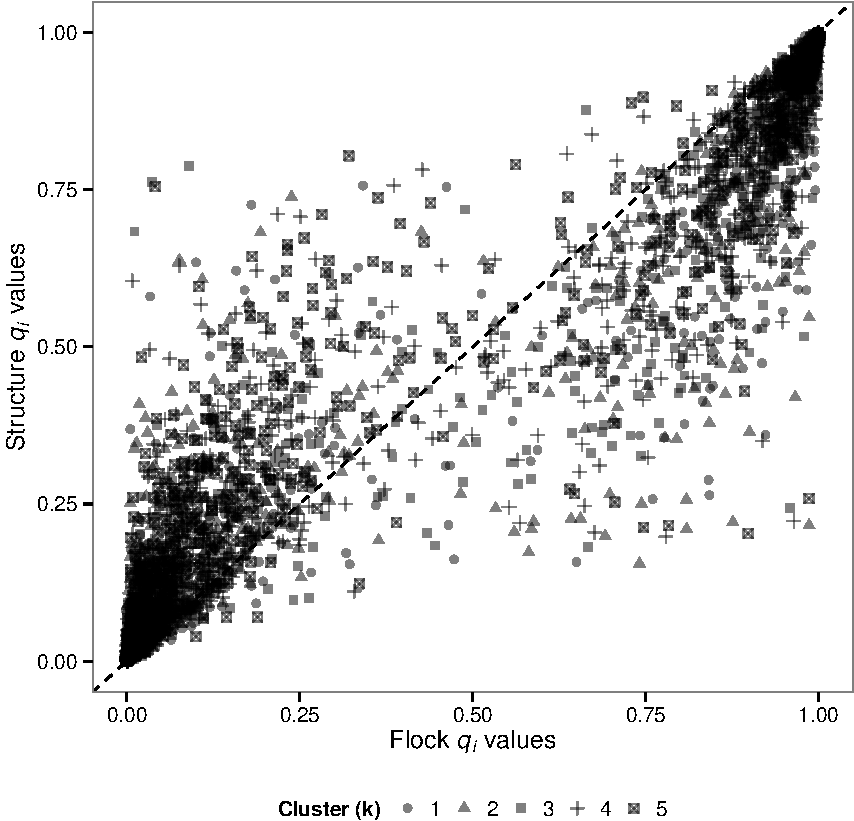
\includegraphics[width=\columnwidth]{images/Figures-Pat/Fig2.pdf}
%    \caption{Individual \textit{$q_i$} values plotted for each cluster for $K=5$. 
%{\sc flock} estimates of likelihood of assignment to each cluster have less uncertainty
% attributed to them.}
%    \label{fig:qscatter}
%\end{center}
%\end{figure}

To investigate the ability of the arrangement of individuals within the reference 
populations to move around the partition space we varied the number of iterations that 
each run goes through to find the ``optimal'' allocation of individuals. Unfortuantely 
only the reallocation matrix for the `best run' is given as output. Increasing the 
number of iterations did not affect the overall inference of $K$. We 
observed that often during the last iterations individuals would alternate between 
reference groups. Increasing the log likelihood 
difference threshold for reallocation to 0.18 (requiring at least a 1.5 times 
higher likelihood to reallocate the individual) minimized this, but did not affect the 
inference of $K$ (lower bound estimate of $K = 2$).

\section*{Conclusions}
In the past decade, the use of genetic markers to identify population structure and to attempt inference of
the number of genetic clusters ($K$) in a collection has dramatically increased in the fields of ecology, evolution, 
epidemiology, and conservation
genetics. The most commonly used program for doing this is {\sc structure} \citep{Pritchardetal2000,Falushetal2003}, 
a full-featured program with many options that is widely-used, well-tested, and reasonably well-understood. 
We've shown here that {\sc flock}, a program that uses a deterministic algorithm, can be regarded
as providing approximate, maximum-{\em a-posteriori} inference from one of the models implemented in 
{\sc structure}. Given the similarities between the two methods, we expect that {\sc flock}
and {\sc structure} (using the no-admixture model with non-correlated allele frequencies) will deliver
similar results.  We observed such similarity in comparing results from {\sc flock} and {\sc structure} 
on a real data set from \textit{O. mykiss} 


Though we observed similar results
between the two programs at low values of $K$, {\sc flock}'s ``best-runs'' solutions became somewhat inconsistent at higher values of $K$, though most solutions were still similar to {\sc structure}'s.
This is likely a consequence of the rapidly increasing size of the search space over possible 
partitions as $K$ and $n$, the number of individuals, increase. 
The likelihood surface defined on partitions of this space will often
be multimodal---possessing numerous local peaks and troughs.
The peak that  {\sc flock}'s deterministic algorithm finds is entirely determined by the initial allocation of 
individuals, as it has no way to visit areas of the surface with smaller likelihood values.
If the number of initial allocations does not increase
as $K$ is increased, the starting allocations become diffusely scattered in the space of all
possible partitions making it less likely that many (if any at all) will converge to the same local mode. This coupled with the fact that there is 
ambiguity in what defines a `best run' when all plateaus are of length zero complicates the interpretation
of results from {\sc flock} if no non-zero plateaus are encountered. Of course, the problem of getting caught in local modes is not unique to {\sc flock}---{\sc structure} itself clearly can wind up sampling predominantly from a fairly isolated part of the space, as evidenced by the different results obtained from different runs of {\sc structure}. 

One of the advantages of {\sc flock} over other methods for genetic clustering
is reported to be the short processing time for each run of {\sc flock}.
While \citet{Duc&Tur2012} observed faster processing times (relative to other methods) in their 
comparisons, we did not observe this advantage in our analysis. This appears to result from two issues. First,
our example data set was an order of magnitude larger than the largest data set analyzed in \citet{Duc&Tur2012}.  
Second, in the comparison by \citet{Duc&Tur2012}, 
{\sc flock} was set to perform 50 runs and 20 iterations for each $K$ starting at 2 and ending when 
one of the stopping conditions was met, and computing times for that analysis were compared to ten iterations of {\sc structure} using 
a 50,000 sweep burn-in followed 
by a 200,000 sweep sample from the posterior for values of $K$ from 1 to three more than the true 
value of $K$. 
To us it seemed reasonable to compare, for each $K$, the running times of one iteration of {\sc structure} (50,000 
burn in and 200,000 sample collection sweeps)
to one iteration of {\sc flock} (50 different starting allocations that are reallocated 20 times) 
as both were used to provide one of 6 total estimates (per value of $K$) of the partition of individuals into 
clusters. In short,
it is difficult to reliably assess differences in program run times when there is no clear consensus on what 
constitutes a reasonable comparison with respect to run length and number of runs.

While there has been lengthy 
discourse over the choice of estimators for $K$ in {\sc structure} 
\citep{Pritchardetal2000,Evannoetal2005,Wap&Gag2006,Gaoetal2011}, less has been written on how the number of 
individuals
and the number of starting allocations can affect not only the convergence of different runs of {\sc flock}, but also its 
inference of $K$. \citeauthor{Duc&Tur2012} developed estimation rules for $K$ based on simulated data 
sets with a modest number of individuals and different migration regimes and rates, numbers of loci, and $K$. 
By relying on the number of identical partitions (mean LLOD values) obtained by {\sc flock} over multiple
runs as a means of supporting 
a particular $K$,  similar---but not identical---partitions
will provide no support to a given $K$. If using {\sc flock}, we advise running
multiple small batches and using the programs {\sc clumpp} \citep{Jak&Ros2007} and
{\sc distruct} \citep{Rosenberg2004} to visually inspect the `best run' results, to determine
if there are many similar-but-not-identical partitions found amongst {\sc flock}'s replicate 
solutions.  

We should point out that our comparison was between {\sc flock} and the {\em no-admixture} model in 
{\sc structure} which is not the default model used in {\sc structure}. Rather, by default, {\sc structure} uses 
its {\em with-admixture} model.  Such a model explicitly tries to account for the admixed origin
of individuals in the sample and thus may be a more appropriate model than the no-admixture model
(or {\sc flock}) when the sample contains individuals that are admixed between populations.  A further advantage
of the with-admixture model is that it allows inferences for the population of origin of individual alleles at 
different loci within individuals, and not just of the individuals themselves.   We also note that {\sc flock} 
corresponds to {\sc structure}'s model with uncorrelated allele frequency priors. \citet{Falushetal2003} found that
using their ``$F$-model,'' which assumes that allele frequencies between populations are correlated {\em a priori}, 
allowed {\sc structure} to dissect more subtle population structure than was possible using the prior with
uncorrelated allele frequencies.  Modifying {\sc flock} so as to reap similar benefits from using a prior
with correlated allele frequencies seems like it would be an interesting challenge, though difficult
because {\sc flock}'s formulation effectively integrates the allele frequencies out of the model.
 


Often, newly-developed algorithms come to be understood within more general contexts and 
frameworks, and this, in turn, can help guide improvement of those algorithms.  For example, in population
genetics, the ``Markov recursion'' algorithm of \citet{Gri&Tav1994-AI} was identified by \citet{Felsensteinetal1999} 
as a special case of importance sampling \citep{Ham&Han1964}, a perspective which allowed 
\citet{Ste&Don2000} to improve upon the algorithm dramatically.  Here we have identified the {\sc flock}
algorithm as a limiting case of simulating annealing upon {\sc structure}'s no-admixture model. We hope this will
help users to understand and interpret {\sc flock}'s behavior and will provide insights that may be useful 
to {\sc flock}'s authors if they further develop their algorithm.   

 
